% -*- TeX:de -*-
\NeedsTeXFormat{LaTeX2e}
\documentclass[12pt,a4paper]{article}
\usepackage[german]{babel} % german text
\usepackage[DIV12]{typearea} % size of printable area
\usepackage[T1]{fontenc} % font encoding
%\usepackage[latin1]{inputenc} % most likely on Windows
\usepackage[utf8]{inputenc} % probably on Linux
\usepackage{multicol}

% PLOTTING
\usepackage{pgfplots} 
\usepackage{pgfplotstable}
\usepackage{url}
\usepackage{graphicx} % to include images
\usepackage{tikz}
\usepackage{subfigure} % for creating subfigures
\usepackage{amsmath} % a bunch of symbols
\usepackage{amssymb} % even more symbols
\usepackage{booktabs} % pretty tables
\usepackage{makecell} % multi row table heading

% a floating environment for circuits
\usepackage{float}
\usepackage{caption}

%\newfloat{circuit}{tbph}{circuits}
%\floatname{circuit}{Schaltplan}

% a floating environment for diagrams
%\newfloat{diagram}{tbph}{diagrams}
%\floatname{diagram}{Diagramm}
\pgfplotsset{compat=1.8}
\selectlanguage{german} % use german

\begin{document}

%%%%%%% DECKBLATT %%%%%%%
\thispagestyle{empty}
			\begin{center}
			\Large{Fakultät für Physik}\\
			\end{center}
\begin{verbatim}


\end{verbatim}
							%Eintrag des Wintersemesters
			\begin{center}
			\textbf{\LARGE SS 14}
			\end{center}
\begin{verbatim}


\end{verbatim}
			\begin{center}
			\textbf{\LARGE{Physikalisches Praktikum\\ für das Bachelorstudium}}
			\end{center}
\begin{verbatim}




\end{verbatim}

			\begin{center}
			\textbf{\LARGE{PROTOKOLL}}
			\end{center}
			
\begin{verbatim}

\end{verbatim}

			\begin{flushleft}
			\textbf{\Large{Experiment (Nr., Titel): PS1 - Schwingungen 1}\\
							%Experiment Nr. und Titel statt den Punkten eintragen
			\LARGE{PS1}}	
			\end{flushleft}

\begin{verbatim}

\end{verbatim}	
							%Eintragen des Abgabedatums, oder des Erstelldatums des Protokolls
			\begin{flushleft}
			\textbf{\Large{Datum:}} \Large{05.06.2014}
			\end{flushleft}
			
\begin{verbatim}
\end{verbatim}
							%Namen der Protokollschreiber
		\begin{flushleft}
			\textbf{\Large{Namen:}} \Large{Patrick Braun, Johannes Kurz}
			\end{flushleft}

\begin{verbatim}


\end{verbatim}
							%Kurstag und Gruppennummer, zb. Fr/5
			\begin{flushleft}
			\textbf{\Large{Kurstag/Gruppe:}} \Large{DO/4}
			\end{flushleft}

\begin{verbatim}

\end{verbatim}
							%Name des Betreuers, das Praktikum betreute.
			\begin{flushleft}
			\LARGE{\textbf{Betreuer:}}	\Large{Wilhelm Markowitsch}	
			\end{flushleft}

%%%%%%% DECKBLATT ENDE %%%%%%%
\pagebreak
\setlength{\columnsep}{20pt}
\begin{multicols}{2}

%%%%%%%%%%%%%%%%%%%%%%%%%%%%%%%%%%%%%%%%%%%%%%%%

%\begin{figure}[H]
%	\centering
%	\includegraphics[scale=0.35]{./data/beugung.png}
%	\caption{Beugungsmuster Einzelspalt (echtes Foto; schwarz durch weiß ersetzt)}
%	\label{fig:beugungsmuster}
%\end{figure}


%\begin{figure}[H]
%	\centering
%	\pgfplotstabletypeset[
%			columns={abstand, n},
%			col sep=&,
%			columns/abstand/.style={precision=2, zerofill, column name=\makecell{$Abstand$\\$(\pm 0.05)[mm]$} }, 
%			columns/n/.style={column name=\makecell{$n$\\$(Ordnung)$}, precision=0},
%			every head row/.style={before row=\hline,after row=\hline\hline},
%			every last row/.style={after row=\hline},
%			every first column/.style={column type/.add={|}{} },
%			every last column/.style={column type/.add={}{|} }
%			]{
%			abstand & n
%			12.9 & 1
%			24.45 & 2
%			37.40 & 3
%			49.35& 4
%			62.45 & 5
%			74.45 & 6
%			87.45 & 7
%			100.25 & 8
%			
%			}
%	\caption{Messwerte Einzelspalt}
%	\label{tab:werte_einzelspalt}
%\end{figure}


%%%%%%%%%%%%%%%%%%%%%%%%%%%%%%%%%%%%%%%%%%%%%%%%
%%%%%%%%%%%%%%%%%%%%%%%%%%%%%%%%%%%%%%%%%%%%%%%%


\section{Schwingungen 1}
In PS1 werden Mechanische Oszillatoren auf ihre Eigenschaften untersucht.
Im Detail werden ein Drehpendel, ein gekoppeltes Pendel und die Dopplerverschiebung ausgemessen. Im folgenden Abschnitt werden die dafür benötigten Grundlagen zusammengefasst.

%%%%%%%%%%%%%%%%%%%%%%%%%%%%%%%%%%%%%%%%%%%%%%%%%%%%%%%%%%%%%%%%%%%%%%%
\subsection{Grundlagen und Versuchsaufbau:}
Grundlage jeder gedämpften harmonischen Schwingung (HS) ist eine ungedämpfte HS. Die kann mit einer Amplitude und einer Winkelfunktion wie folgt beschrieben werden:
$$f(t) = A \cdot cos(\omega t + \phi)$$
Hierbei ist \textbf{A} die Amplitude, \textbf{$\omega$} die Kreisfrequenz, \textbf{t} die Zeit und \textbf{$\phi$} die Phase mit der die Schingung begonnen hat (zu t=0).\\
Betrachtet man nun eine gedämpfte Schwingung ergibt sich aus der Differentialgelichung [1](2, p.4) ein zusätzlicher zeitabhängiger Dämpfungsterm: 
$$f(t) = A \cdot e^{- \delta t} \cdot cos(\omega t + \phi)$$ 
Hierbei ist $\delta$ die Dämpfungskonstante welche vom Material (z.B. Luft, Eisen) und anderen Bedingungen abhängt (z.B. Kugellager, Reibung etc.).\\

Eine reale Schwingung ist nie ungedämpft. Würde es eine ungedämpfte Schwingung geben, könnte die so genannte Resonanzkatastrophe auftreten. Hierbei würde bei einer erzwungenen Schwingung mit der Resonanzfrequenz getrieben und immer mehr Energie auf das schwingende System übertragen bis diese über alle Grenzen anwächst.\\
Um einen Oszillator zu beschreiben wird die \textbf{Eigenfrequenz} verwendet. Diese entspricht der Kreisfrequenz bei einer Schwingung ohne dämpfung und wird im Weiteren als $\omega_0$ bezeichnet.\\

\textbf{Drehpendel}
Zur charakterisierung des Drehpendels wird durch das logarithmische Dämpfungsdekrement $\Lambda$ der Dämpfungskoeffizient berechnet:
$$\Lambda = ln \frac{x(T_1)}{x(T_2)} = \delta T$$
Dabei wird die Änderung der Amplitude bei aufeinander folgenden Perioden betrachtet ($\frac{x(T_1)}{x(T_2)} = e^{\delta T}$).\\
Die Eigenfrequenz wird wie folgt unter Berücksichtigung von $\delta$ berechnet:
$$ \omega_0 = \sqrt{\frac{2\cdot \delta \omega}{tan \phi} + \omega^2 }$$
Eine zweite Möglichkeit die Eigenfrequenz zu bestimmen ist die Resonanzkurve einer erzwungenen Schwingung zu ermitteln und die Halbwertsbreite bei $\frac{A}{\sqrt{2}}$ zu messen (vgl. [1](9, p.6)).\\
Ein weiteres Maß für einen Oszillator ist der Gütefaktor Q. Dieser ist definiert als:
$$Q = \frac{\omega_0}{2\delta} = \frac{\omega_0}{\Delta \omega}$$

\textbf{Gekoppelte Pendel}
Bei einem gekoppelten Pendel beeinflussen sich wechselseitig zwei Pendel welche miteinander verbunden sind. In Abbildung \ref{fig:gekoppelt_skizze} sind die wesentlichen Eigenschaften der Kopplung zu sehen.

\begin{figure}[H]
	\centering
	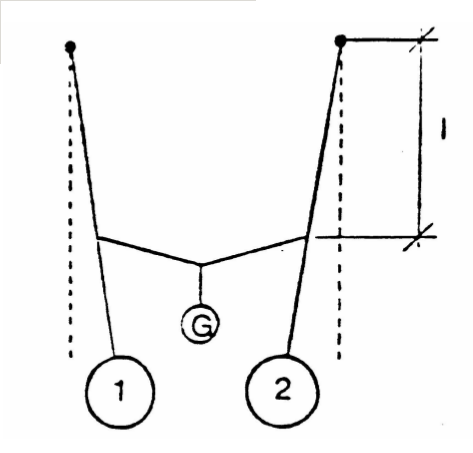
\includegraphics[scale=0.4]{./figure/skizze_kopplung.png}
	\caption{Skizze eines gekoppelten Pendels [1](Abb.7, p.9)}
	\label{fig:gekoppelt_skizze}
\end{figure}
Die kopllungslänge \textbf{l} und das Gewicht \textbf{G} beeinflussen die Schwingung des Gesamtsystems. Je nach Anfangsbedingungen kann man drei Fälle unterscheiden:\\
\begin{itemize}
	\item  \textbf{Gleichsinnige Schwingung} \\ beide schwingen mit $\omega_0$
	\item  \textbf{Gegensinnige Schwingung} \\ kopplungsabhängige höhere Frequenz
	\item  \textbf{Schwebungsfall} \\ abwechselnd Schwingung und Stillstand
\end{itemize}

%%%%%%%%%%%%%%%%%%%%%%%%%%%%%%%%%%%%%%%%%%%%%
% TODO genauer ausformulieren + formeln
%%%%%%%%%%%%%%%%%%%%%%%%%%%%%%%%%%%%%%%%%%%%%

\textbf{Dopplerverschiebung einer bewegten Schallquelle}
Bei der Bestimmung der Schallgeschwindigkeit wird der Schwebungsfall des Doppelpendels verwendet. Anhand der Schwebungsdauer von zwei gleichen Schallquellen (eine in Bewegung), der Frequenz und der Relativgeschwindigkeit kann die Schallgeschwindigkeit in Luft wie folgt errechnet werden:
$$c_{Luft} = \frac{v}{\frac{\nu}{\nu_0}-1}$$
$\nu_0$ \ldots die Frequenz der Schallquelle\\ 
$\nu$ \ldots die durch den Dopplereffekt veränderte Frequenz\\
$v$ \ldots Bewegungsgeschwindigkeit\\
\\
Trägt man $\Delta \nu / \nu_0$ gegen v auf, entspricht der Anstieg der Schallgeschwindigkeit.

\pagebreak
%%%%%%%%%%%%%%%%%%%%%%%%%%%%%%%%%%%%%%%%%%%%%%%%%%%%%%%%%%%%%%%%%%%%%%%
\subsection{Resultate}
\textbf{Drehpendel}

\begin{figure}[H]
	\centering
	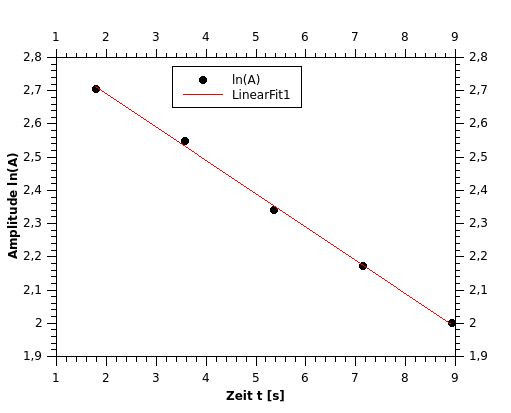
\includegraphics[scale=2]{./figure/Messung1_Daempfung_omega0.png}
	\caption{Bestimmung des Dämpfungskoeffizienten Dämpfung 1 (250mA)}
	\label{fig:daempfung_omega0_1}
\end{figure}

% TODO grafik von Pats QTI 
\begin{figure}[H]
	\centering
	%\includegraphics[scale=0.8]{./figure/Messung2_Daempfung_omega0.png}
	\caption{Bestimmung des Dämpfungskoeffizienten Dämpfung 2 (350mA)}
	\label{fig:daempfung_omega0_2}
\end{figure}

\end{multicols}

\begin{figure}[H]
	\centering
	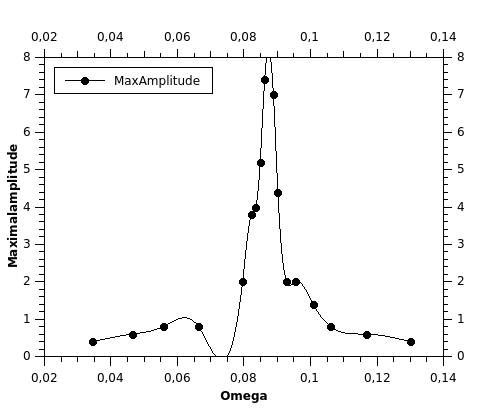
\includegraphics[scale=1.5]{./figure/Messung1_Resonanzkurve_250mA.png}
	\caption{Resonanzkurve (250mA)}
	\label{fig:resonanzkurve_250mA}
\end{figure}
Halbwertsbreite: 3.5404 - 3.3584 = 0.182 \pm 0.001

\begin{multicols}{2}

\textbf{Gekoppelte Pendel}



\textbf{Dopplerverschiebung einer bewegten Schallquelle}
Von Beobachter weg:\\
B (y-intercept) = 2,169943820978748e-02 +/- 1,351263299960912e-01\\
A (slope) = 5,036956678235092e+01 +/- 3,421154601278228e+00\\

Zum Beobachter:\\
B (y-intercept) = 4,178049407699678e-01 +/- 1,566248245895523e-01\\
A (slope) = 3,702851334267199e+01 +/- 3,536858402679127e+00\\

% \begin{figure}[H]
% 	\centering
% 	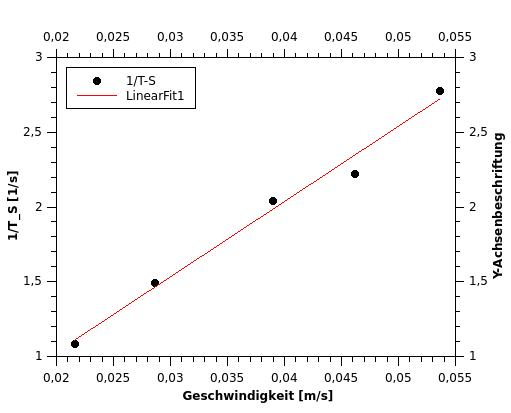
\includegraphics[scale=0.8]{./figure/Aufgabe3_weg_von_Beob.png}
% 	\caption{ Weg von }
% 	\label{fig:weg_von}
% \end{figure}
\begin{figure}[H]
	\centering
	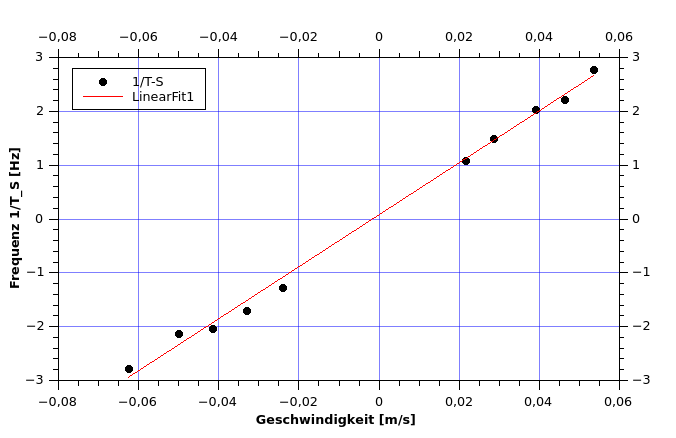
\includegraphics[scale=1.2]{./figure/Dopplereffekt.png}
	\caption{Dopplereffekt lin. Regression mit bewegtem Beobachter in beide Richtungen}
	\label{fig:doppler}
\end{figure}



\pagebreak
%%%%%%%%%%%%%%%%%%%%%%%%%%%%%%%%%%%%%%%%%%%%%%%%%%%%%%%%%%%%%%%%%%%%%%%
\subsection{Diskussion}
\textbf{Drehpendel}

\textbf{Gekoppelte Pendel}

\textbf{Dopplerverschiebung einer bewegten Schallquelle}


\section{Quellen}
$[1]$ Anleitung, \url{http://www.univie.ac.at/anfpra/neu1/ps/ps1/PS1.pdf}\\
$[2]$ Rohdaten, \url{htts://github.com/blackandcold/Protocols-SS2014-P2/tree/master/PS_1/data}\\

\end{multicols}
\end{document}